\newpage
\section{Problem}

The goal of this project is to create a user-friendly application that can generate modern 3D cities, and then export them as \textit{.fbx} files.
\textit{User-friendly} means that users should not need any technical expertise or coding experince to fully utilize the application.
\textit{Modern cities} will in this project be defined as cities that resemble
modern industrialized cities such as New York, Paris, San Francisco, and Tokyo.
Figure~\ref{fig:ModernCities} showcases two examples of such modern cities.

\begin{figure}[h!]
  \centering

  \begin{subfigure}[b]{0.48\textwidth}
    \frame{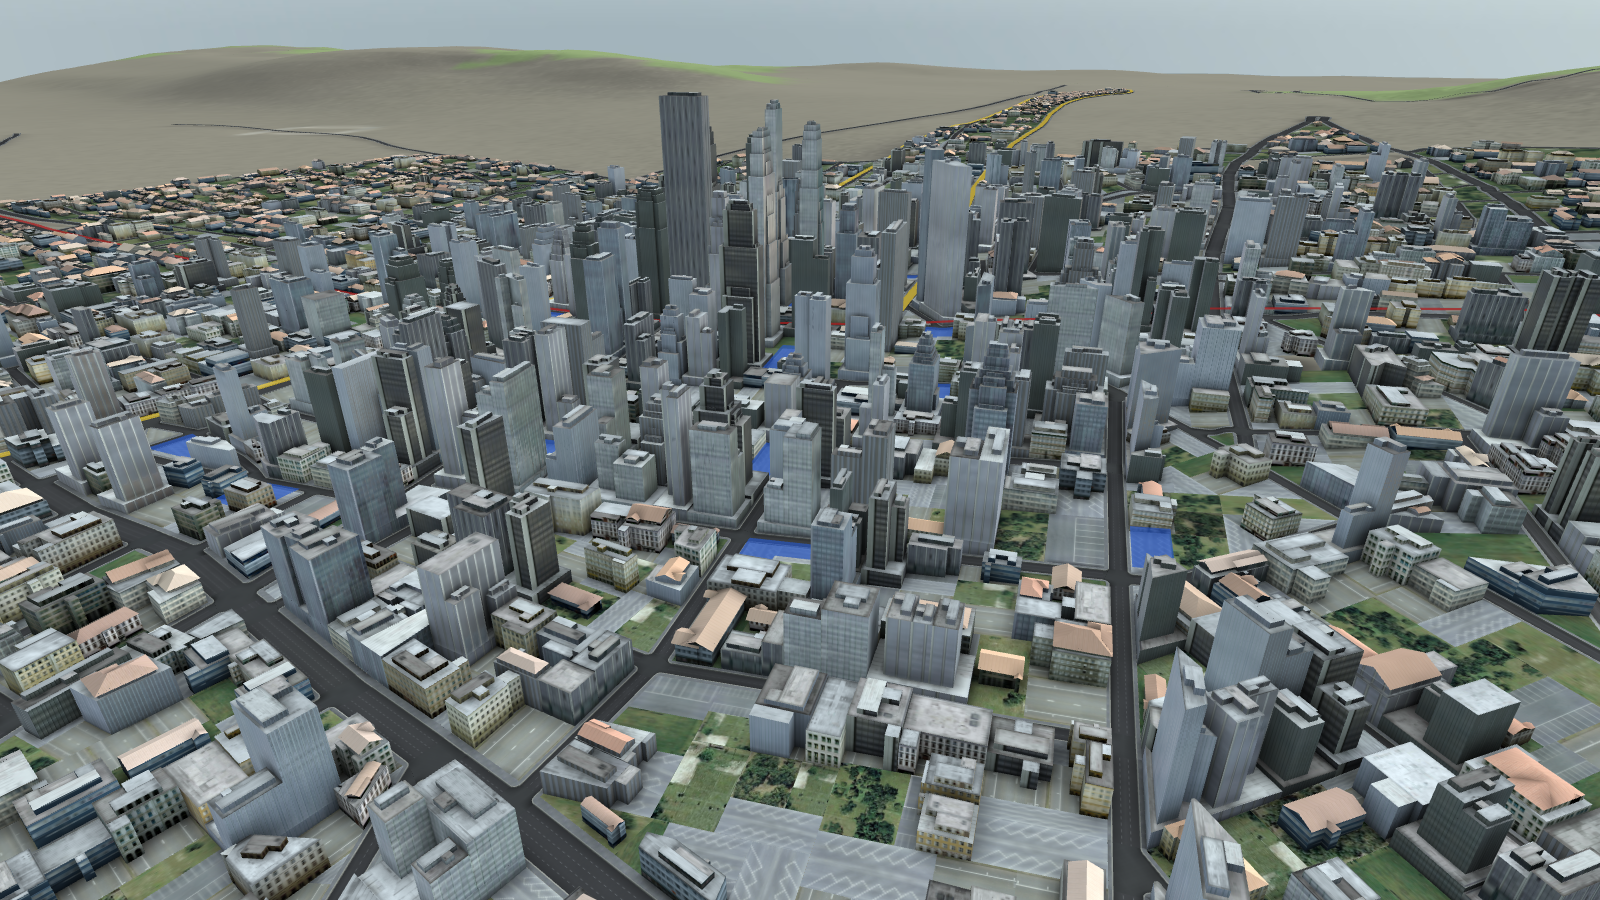
\includegraphics[width=\textwidth]{figure/modern-city.png}}
  \end{subfigure}
  \quad
  \begin{subfigure}[b]{0.48\textwidth}
    \frame{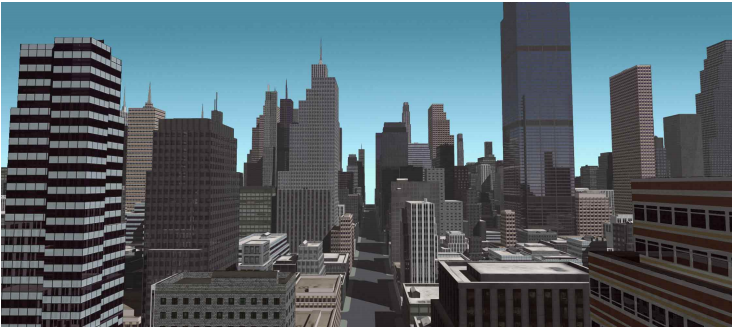
\includegraphics[width=\textwidth]{figure/modern-city2.png}}
  \end{subfigure}

  \caption{Examples of generated modern cities from related works \cite{yoav_and_pascal}\cite{cl3ver}.}
  \label{fig:ModernCities}
\end{figure}

It is worth clarifying that suburban areas and rural areas are also included as
part of such cities.

The scope will be restricted to generating static models that can be exported as \textit{.fbx} files.
Therefore, dynamic content such as simulation of road traffic, day-night cycle,
and pedestrians are all considered out of scope for this project.
The interior of buildings are also considered out of scope.
The reason being that each user is predicted to have fairly unique intentions with 
what content they want to fill the buildings with. This feature would likely not
fit the project's time frame either.

The primary focus will be put on the generation of roads and buildings, as these
are considered the core features of a city.
The terrain's purpose should be to help create natural
settings for the infrastructure to adjust to, and the terrain itself does not need
to have realistic level of detail. Furthermore, the details of roads and
buildings, such as textures and small meshes, are not intended to be made from
scratch. Utilization of free resources online is encouraged to keep the workload
focused on algorithmic problems rather than on 3D modeling.

As a consequence of the random aspect in PCG, it is difficult to express a precise definition that can measure whether the project should be considered successful or not.
One possible measurement is the \textit{quality} of the exported models.
Do the cities look like real ones?
Are they visually pleasing and are they suitable for use in other mediums such as movies and games?
Another possible measurement is how \textit{expressive} the generation is.
If all generated models look exactly the same, then the power of PCG has gone unused.
Each generated model should stand out, and it should not be apparent whether a
human or a computer made them.

The subjective nature of these measurements will make evaluation challenging,
but they can still be used to give a rough estimate.
The plan is to measure all of the mentioned aspects from the perspective of
the project members, the project's supervisor, and from a sample of unrelated
university students. This will be done through a survey at the end of the project.

The user will interact with the application's Graphical User Interface (GUI) in the following way.
\begin{enumerate}
  \item The user specifies the size of the world in terms of a 2D plane.
  \item The user specifies any optional parameters that affect the terrain
    such as sea level.
  \item The user clicks on a button that says ``Generate Terrain'' as many times
    as they like, until they are satisfied with the generated terrain.
  \item The user selects which region of the generated terrain they want to use in the final model.
  \item The user places population markers on the terrain and specifies how much
    population each marker represents. The user can also specify any optional
    parameters for each marker such as road type.
  \item The user clicks on a button that says ``Generate Roads'' as many times
    as they like, until they are satisfied with the generated road network.
  \item The user clicks on a button that says ``Generate Buildings'' as many times
    as they like, until they are satisfied with the generated buildings.
  \item Finally, when the user is satisfied with the result they can click on a
    button that says ``Export to FBX'' and the the program will save the full
    model as a \textit{.fbx} on the local file system.
\end{enumerate}

As a stretch goal, the user should after step 7 be able to select blocks of a
city and regenerate those individually. With such a feature in place, the user
would be able to finely adjust parts of the generation to their preference. This
feature would not require any additional mandatory steps for the user to take.

The problem addressed in this project can be divided into 3 major subproblems:
terrain generation, road generation, and building generation.
Each of the following subsections will go into more detail about these
subproblems.

\newpage
\subsection{Terrain Generation}

The problem of terrain generation can be further divided into the following tasks.
\begin{easylist}
  @ Generate the heights of the terrain.
  @ Texture the terrain based on height levels.
  @ Generate trees and shrubs.
  @ Generate ocean.
  @ Generate lakes.
  @ Generate rivers that flow into lakes and the ocean. (optional)
\end{easylist}

The terrain heights need to represent the hills and valleys that define the silhouette of the world.
The textures should aid in visually describing the landscape, as well as
help contribute to an overall more realistic model. The following list presents
a few concrete examples of such texturing.
\begin{easylist}
  @ Oceans and lakes should have a blue tint.
  @ Landscape slanting towards oceans should transition into beaches.
  @ Spacious plains should cover various shades of green.
  @ Mountains should appear rocky.
  @ Tall mountain peaks should be covered in snow.
\end{easylist}

In the context of realism, the generation should assume a season somewhere
between spring and summer.
This scope could potentially be extended to include other seasons as well as
different types of landscape types.
However this is only intended as an optional aspect that will handled in the case
of excess time.

To make the terrain more convincing there will also be generation of trees and shrubs
throughout the world. These should grow in groups, just like forests in
real life, and they should not intersect with any roads or buildings.

The generated lakes and oceans will both restrict where roads and buildings can be placed.
The same goes for rivers if that strech goal is met.
These aspects should help create more interesting interactions between terrain and city.

The overall terrain should follow a realistic aesthetic. Consequently it should not
attempt follow a \textit{Low Poly} aesthetic nor be made up of visible \textit{Voxels}.
\newpage
\subsection{Road Generation}
\newpage
\subsection{Building Generation}

The problem of building generation can be further divided into the following tasks.

\begin{easylist}
  @ Generate different types of buildings depending on population.
  @ Generate villas.
  @ Generate terraced houses.
  @ Generate apartments.
  @ Generate skyscrapers.
  @ Generate parks.
  @ Generate stores, restaurants, hotels, and more. (stretch goal)
\end{easylist}

The relation between population and building types does not be realistic in
terms of scale, but there should be a clear positive correlation.
Areas with metropolitan-levels of population should have a high frequency of skyscrapers, apartments, and other tall buildings.
Medium-density areas should contain apartments and terraced houses, while low
density areas should mostly contains villas.

Other buildings such as stores and restaurants would help enrich the cities with
more variety, but they might require a lot of time spent on modeling.
Because of this they have been defined as stretch goals.
However there are no restrictions on the appearance of any buildings (even the
mandatory ones) as long as they have clear real-life equivalents.

Although parks are not technically buildings, they will be included here for the
sake of brevity and because of their similarity.
Like buildings, parks will vary depending on population density.
In high-density areas they should occur relatively frequently, especially large
ones, but the they should slowly be replaced by areas of nature as one approaches the outskirts.
